Sensory termoelektryczne wykorzystują zjawisko termoelekryczne, nazywane też efektem
Seebecka.~W~obwodzie, który składa się~z~dwóch różnych metali, których końce są połączone~i~znajdują
się~w~różnych temperaturach, płynie prąd elektryczny. Jednakże~w~celu pomiarów temperatury wymagany
jest pomiar różnicy potencjałów (spadku napięcia), pojawiającego się między niepołączonymi końcami
przewodników. Schemat układu do wykonywania takiego pomiaru przedstawiono na rysunku
\ref{img:thermocouple}. Zmierzona różnica potencjałów wyraża się równaniem:

\begin{equation}
  \Delta \varphi = S_{AB}\cdot\Delta T
\end{equation}

\begin{eqparams}
  S_{AB} & współczynnik Seebecka,~w~temperaturze 0\degC, \\
  \Delta T & różnica temperatur pomiędzy stroną \enquote{gorącą} oraz \enquote{zimną} układu.
\end{eqparams}

\begin{figure}[!htbp]
  \centering
  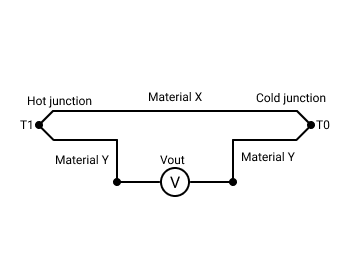
\includegraphics[scale=0.8]{sensor-theory/temperature-thermocouple}
  \caption{\label{img:thermocouple}Schemat sensora termoelektrycznego -- termoogniwa}
\end{figure}

Współczynnik Seebecka jest wartością charakterystyczną dla danego typu termoogniwa, zależnym od
metali, które zostały użyte do wytworzenia sensora. Wartości współczynnika \cite{thermocouple} dla
wybranych termoelementów wraz~z~ich oznaczeniami przedstawia tabela \ref{tab:thermocouple}.

\begin{table}[!htbp]
  \centering
  \caption{\label{tab:thermocouple}Wartości współczynnika Seebecka dla wybranych termoogniw}
  \begin{tabular}{ccc}
    \toprule
    Typ termoogniwa & Oznaczenie & Współczynnik Seebecka $S_{AB}$ [$\mu V\cdot$\degC$^{-1}$] \\
    \midrule
    Fe-CuNi         & J          & 51                                                        \\
    NiCr-NiAl       & K          & 40                                                        \\
    PtRh(13\%)-Pt   & R          & 12                                                        \\
    Cu-CuNi         & T          & 60                                                        \\
    NiCr-CuNi       & E          & 40                                                        \\
    \bottomrule
  \end{tabular}
\end{table}